\documentclass[french, 11pt, a4paper]{article} %langue française, police 11pt, format A4
\usepackage[french]{babel} % français, notamment pour la date, les défs, les thm., etc.
\usepackage[T1]{fontenc}
\usepackage{geometry} % pour les marges
\usepackage{array} % pour écrire l'application \phi en conclusion
\usepackage{amstext} % pour /text dans le mode math
\usepackage{amsmath} % pour les grandes fractions
\frenchsetup{StandardLists=true} % pour 'itemize' : des bullets et des interlignes pour une meilleure clarté
\usepackage{enumitem} %idem
\usepackage{amssymb} % pour les divers symboles, notamment \mathbb{}
\usepackage{stmaryrd} % pour les intervalles entiers
\usepackage{verbatim} % pour le formattage "mono"-like. Utilisation : \verb+TexteAFormatter+
\usepackage{listings}
\usepackage{xcolor}
\usepackage{graphicx}
\usepackage{makecell} % pour plusieurs lignes dans les cellules d'un tableau
\geometry{hmargin=1.3cm,vmargin=2cm} % marges élargies

%%% nouvelles commandes pour alléger l'écriture %%%

%% en mode math !! (entre des '$ $')
\newcommand{\Sc}{\mathcal{S}} % '\F' pour un F cursif
\newcommand{\N}{\mathbb{N}}
\newcommand{\R}{\mathbb{R}^*_+}
\newcommand{\ra}{\rightarrow}

%% en mode text
\newcommand{\smb}{\smallbreak}


%% en-têtes
\title{Projet : Un problème de tournée de drones dans un contexte de déconfinement}
% corriger saut de ligne pour les auteurs
\author{PREKA Bruno, ZELLE Lars Yannick (681C)}
%% \date{\today}

%% début
\begin{document}


\maketitle



\section{Introduction}

Dans le contexte sanitaire actuel, un scénario fictif suggère l'isolement \emph{total} des personnes
atteintes de la Covid-19 dans leur domicile. Des drones sont alors réquisitionnés pour livrer des courses
à domicile.
\smb Dans chaque zone géographique, un unique dépôt (qu'on notera $1$ par la suite) stocke des ressources alimentaires et médicamenteuses.
Plusieurs contraintes se dessinent dans ce problème appartenant à la classe des problèmes de tournées de véhicules.
La contrainte garantissant que chaque client est visité une seule fois, ainsi que celle de la charge supportée par un drone,
y interviennent.
Le but du problème est de minimiser la distance parcourue par l'ensemble des drones.
\smb On résout ce problème à travers deux méthodes possibles :
\vspace{-0.2cm}
\begin{enumerate}
    \item Dite \emph{exacte}, la méthode fait appel à un problème d'optimisation
combinatoire, mais qui peut demander un temps d'exécution très important aux yeux des décideurs ;
    \item \emph{Approchée}, celle-ci est une variante de l'heuristique de Clark et Wright.
\end{enumerate}

\subsection{\emph{Lisez-moi}}
\begin{itemize}
    \item Pour lancer la résolution exacte sur une instance de chemin \verb+pathToMyInst.dat+, il faut entrer successivement
    les commandes suivantes:
        \begin{itemize}
            \item \verb+include("Projet_ResExacte.jl")+
            \item \verb+timer_res_exact("pathToMyInst.dat")+
        \end{itemize}
    \item Quant à la résolution approchée, seul l'appel à la fonction de résolution change : \\ \verb+data_then_solve_appr("pathToMyInst.dat")+
\end{itemize}


\subsection{Structures de données générales}

\subsubsection{Données du problème}
A partir de la fonction \verb+lecture_donnees+, on traduit les instances numériques fournies
par la structure de données 
\verb+donnees+ dont les champs sont dédiés au nombre de clients \verb+nbClients+ (y compris le dépôt), à
la \verb+capacité+ du drone, à la \verb+demande+ des clients et au distancier \verb+distance+. On retrouvera régulièrement les types suivants :
\begin{itemize}
    \item \verb+nbClients+ $=:n$ et \verb+capacite+ sont des entiers. Par la suite, tous les entiers seront de type \verb+Int64+ ;
    \item \verb+demande+ est un vecteur d'entiers \verb+Vector{Int64}+ : la demande du client $i$ est renseigné dans la case \verb+demande[+$i$\verb+]+, ce qui facilitera son accès.
    \item \verb+distance+ est une matrice à coefficients entiers \verb+Matrix{Int64}+. Ce type est équivalent à \verb+Array{Int64,2}+, ce qui sera utile pour manipuler des sous-matrices (restrictions de matrice).
\end{itemize}

\subsubsection{Ensemble des regroupements possibles : \texttt{S} $ = \Sc$}
On rappelle que l'ensemble des regroupements possibles est défini par :
\[\Sc := \Bigg\{ S \subseteq \llbracket 2,n \rrbracket : \sum_{j \in S} d_j \leq capacite \Bigg\} \]
\smb Il est clair que la manipulation d'ensembles (type \verb+Set+) est simple, mais elle demande des temps d'exécution plus importants.
Il est donc plus que nécessaire de recourir à un "vecteur de vecteurs" au lieu d'un "ensemble d'ensembles", d'où
le type \verb+Vector{Vector{Int64}}+ pour l'ensemble des regroupements.

\subsubsection{Ensemble d'ensembles d'indices de tournées visitant le $i$-ème client : \\ \texttt{AllS\_i} $= \{S_i \subseteq \llbracket 1, |\Sc| \rrbracket \: : \: \forall j \in S_i, \: i \in tournee_j\}_{i \in \llbracket 2 , n \rrbracket }$ }
La contrainte garantissant que chaque client soit visité une seule fois est donnée par :
\[ \sum_{j \in S_i} x_j = 1, i \in \llbracket 2,n \rrbracket, \]
où $S_i \subseteq \llbracket 1, |\Sc| \rrbracket$ est le sous-ensemble d'indices des tournées
contenant le client $i$.
Pour les mêmes raisons que ce qui précède, on opte pour un vecteur de vecteurs d'entiers, au lieu d'un ensemble d'ensembles d'entiers,
d'où le type \verb+Vector{Vector{Int64}}+.
\smb Pour un client $i$, l'accès à l'ensemble des indices des tournées le desservant se fait par \texttt{AllS\_i[}$i$\verb+]+ $=S_i$.

\subsubsection{Association tournée-distance minimale : \\ \texttt{l} 
$= \{(tournee_j,l_j) \: : \: \forall j \in \llbracket 1,|\Sc| \hspace{-0.15cm} \rrbracket,  \:
tournee_j \in \Sc 
\: \land \:
l_j = \min_{\text{\normalfont{TSP}}} \text{\normalfont{dist}}(tournee_j) \}$}

A minimiser, la fonction objectif s'écrit :
\[ z = \sum_{j=1}^{|\Sc|} l_j x_j,\]
où $l_j$ désigne la distance minimale du regroupement $j \in \llbracket 1,|\Sc| \rrbracket$, calculée par la
fonction \verb+solveTSPExact+ de résolution du problème de voyageur de commerce (dit TSP, pour \emph{Travelling Salesman Problem}).
Ainsi, une telle expression requiert de lier cette distance à son regroupement via un accès immédiat.
C'est pourquoi, le vecteur \verb+l+ est constitué de couples $(tourn \text{é} e,distance_{\text{min}})$.
Il est de type \verb+Vector{Tuple{Vector{Int64},Int64}}+.
\smb Enfin, en termes d'accès, on a : $\forall j \in \llbracket 1,|\Sc| \rrbracket, \: l_j = $ \texttt{l[j][2]}.


\section{Résolution exacte}
\subsection{Fonction d'énumération des regroupements possibles des clients}
On appelle cette fonction \texttt{getSubsets\_recursive(P,S,capacite,demande,index,d,distances)},
où : \begin{itemize}
    \item \verb+P+ et \verb+toadd+ sont les vecteurs des indices à ajouter pour compléter un regroupement, \verb+toadd+ étant une copie de \verb+P+ ;
    \item \verb+S+ est l'ensemble des regroupements ;
    \item \verb+capacite+ désigne la capacité du drone ;
    \item \verb+demande+ est le vecteur de la demande des clients ;
    \item \verb+index+ est un curseur ;
    \item \verb+d+ est l'accumulateur courant de la demande pour respecter la condition de $\Sc$ ;
    \item \verb+distances+ est le distancier.
\end{itemize}

Derrière cette fonction, l'algorithme consiste à itérer (via $i:=$ \verb+index+) sur toutes les demandes des clients
et à vérifier si la demande du client $i \in \llbracket 2,n \rrbracket$, accumulée à \verb+d+, est conforme à la capacité. Ainsi,
pour le client $i$ : 
\begin{enumerate}
    \item Si les demandes sommées sont en-dessous du seuil, on sauvegarde l'ensemble \verb+P+ des clients à ajouter dans \verb+toadd+
    et on ajoute le client suivant $i+1$ (à ajouter) à \verb+toadd+. Sinon, rien n'est fait et on passe à l'étape 4.
    \item On construit l'ensemble \verb+S+ $= \Sc$ en concaténant/réunissant \verb+S+ et \verb+[toadd]+.
    \item On répète le processus sur \verb+S+ et le client suivant $i+1$ et on compare le nouvel ensemble \verb+Snew+
    de regroupements : si \verb+Snew+ accueille de nouveaux regroupements, alors on les ajoute à \verb+S+.
    \item Une fois ce processus récursif terminé sur ce sous-groupe de clients $\{i,i+1,...,n\}$, on recommence pour le client $i+1$ et le sous-groupe
$\{i+1,...,n\}$.
\end{enumerate}
\smb Par conséquent, il en résulte l'ensemble des regroupements attendu, à savoir $\Sc = $ \verb+S+.
\smb La fonction \texttt{getSubsets(capacite,demande,distances)} vient encapsuler la fonction récursive par l'appel
\texttt{getSubsets\_recursive([],[],capacite,demande,1,0,distances)}, avec \verb+index+ $=1$ et la distance \verb+d+ initialisée à $0$.

\subsection{Fonction déterminant la tournée et sa distance minimale dans un regroupement \texttt{Si}}
On appelle cette fonction \texttt{determineShortestCycle(Si,d)}, où : 
\begin{itemize}
    \item \verb+Si+ est un regroupement de clients à visiter (de type \verb+Vector{Int64}+) ;
    \item \verb+d+ est le distancier (\verb+Matrix{Int64}+).
\end{itemize}
\smb Puisque \verb+Si+ $\subseteq \llbracket 2,n \rrbracket$, il n'inclut pas le dépôt $1$. Ainsi, la réunion avec $\{1\}$
est primordiale pour passer par la fonction \verb+solveTSPExact(d)+ de résolution du TSP.
\smb De plus, il faut restreindre \verb+d+ au regroupement donné, d'où une sous-matrice
\verb+newd = d[Si,Si]+. Une telle opération est permise par l'équivalence entre les types
\verb+Matrix{.}+ et \verb+Array{.,2}+, comme évoqué précédemment.
\smb \verb+solveTSPExact+ retourne alors un couple $(tourn\text{é}e,dist_{\text{min}})$. Néanmoins, elle ne raisonne pas sur l'ensemble d'indices \verb+Si+, mais bien sur
$\llbracket 1,|\text{\texttt{Si}}| \rrbracket$. 
\smb Un réajustement des indices doit conserver la cohérence
des indices dans les tournées. Pour ce faire, on sait que le premier indice traité par \verb+solveTSPExact+ correspond au premier de \verb+Si+,
idem pour le deuxième, ainsi de suite... Puis, dans l'ordre, on a les correspondances suivantes :
\begin{itemize}
    \item le premier client $k_1$ de $tourn\text{é}e \longrightarrow$ client d'indice $k_1$ dans \verb+Si+ ;
    \item \dots
    \item le $i$-ème client $k_i$ de $tourn\text{é}e \longrightarrow$ client numéro \verb+Si[+$k_i$\verb+]+
    \item \dots
\end{itemize}

Ces correspondances donnent lieu à la "nouvelle" tournée, nommée \verb+newtournee+, qui est retournée.

\section{Résolution approchée}

Dans les grandes lignes, on a opté pour les points algorithmiques suivants dans le cadre de l'heuristique de Clark et Wright :

\begin{enumerate}
    \item On conserve le format vectoriel pour écrire une tournée : $[1,...,1]$ qui signifie $1 \ra ... \ra 1$ ;
    \item Initialement, on munit la fonction \verb+getAllFusionnedCycles+ de fusion du vecteur des tournées élémentaires $1 \ra i \ra 1$ 
    (cf \verb+initialiserChemins+)
    et du vecteur des gains $((i,j),g_{ij})$ (cf \verb+calcGainVector+), avec $i,j \in \llbracket 2,n \rrbracket, i \neq j$.
    Par ailleurs, on opte pour un vecteur de couples, sans passer par une matrice de gains, car on veut simplifier le tri décroissant par gains et les accès aux fusions
    possibles ;
    \item Pour chaque itération, on cherche à fusionner deux chemins compatibles (comme imposé dans le sujet). 
        Mais, si la fusion a lieu, il faut garder l'information comme quoi on a fusionné ces 2 chemins !
        \\ Exemple : soit la fusion possible $(2,4)$ qui donne $1 \ra 2 \ra 4 \ra 1$. 
        Que se passe-t-il si, à l'itération suivante, on regarde la fusion $(4,8)$ ? 
        Il faut que l'on sache que $4$ est déjà dans la solution $1 \ra 2 \ra 4 \ra 1$ ;
    \item On a alors besoin d'une structure de données qui conserve, pour chaque chemin, 
    l'information qui indique si ce chemin a déjà été fusionné avec un autre. 
    \\ Ainsi, on joint à chaque chemin un entier,
    disons $0$ si le chemin n'a jamais fusionné dans un autre ; $k \in \N^*$ s'il a été utilisé pour être fusionné avec le $k$-ème chemin.
    \\ Dans l'implémentation, cela se traduit par le vecteur \verb+sol+ de couples $(chemin,k)$, 
    avec $k \in \N$ qui respecte la condition citée précédemment. En Julia, \verb+sol+ est de type \texttt{Vector\{Tuple\{Vector\{Int64\},Int64\}\}} ;
    \item Après une itération (ou une fusion), il reste encore des fusions à traiter, qui ne sont pas encore intervenues dans un chemin. 
    C'est pourquoi, la fonction \verb+removeFusion+ a pour but de minimiser le nombre d'itérations 
    et celui des accès au vecteur de gains.
    \\ Pour cela, si une fusion a lieu (i.e. compatible) et si le chemin en résultant est de taille supérieure à $4$ 
    (en effet si $[1,i,1]$ et $[1,j,i]$ sont fusionnés, alors il n'y a rien à faire : $[1,i,j,1]$), 
    i.e. le chemin est de la forme $[1,\underbrace{a,...,i,j,...,b}_{\text{taille} ~>~ 4},1]$, alors on supprime tous les couples 
    $(a,b), (\_,j), (i,\_), (j,\_), (\_,i)$ qui restent à traiter dans la liste des fusions possibles. Le détail de la disjonction de cas
    peut être directement lu dans le code.
\end{enumerate}

\section{Analyse des résultats issus des instances numériques ($A$ et $B$) pour la méthode \emph{exacte}} 

Les tests ont été réalisés sur une configuration Ubuntu, épaulée d'un processeur double-coeur (à 4 threads) Intel Core i3 cadencé à 2,3 GHz et de 12 GB de RAM.

A l'aide de la macro \texttt{@time} de Julia, on a mesuré les temps d'exécution (en secondes) des fonctions principales et les allocations mémoires.
Par ailleurs, on a également récupéré le nombre de regroupements pour chaque instance et les tailles minimale et maximale des regroupements.
Ces résultats sont donnés par les tableaux suivants :

\subsection{Instances $A$}

\begin{center}
    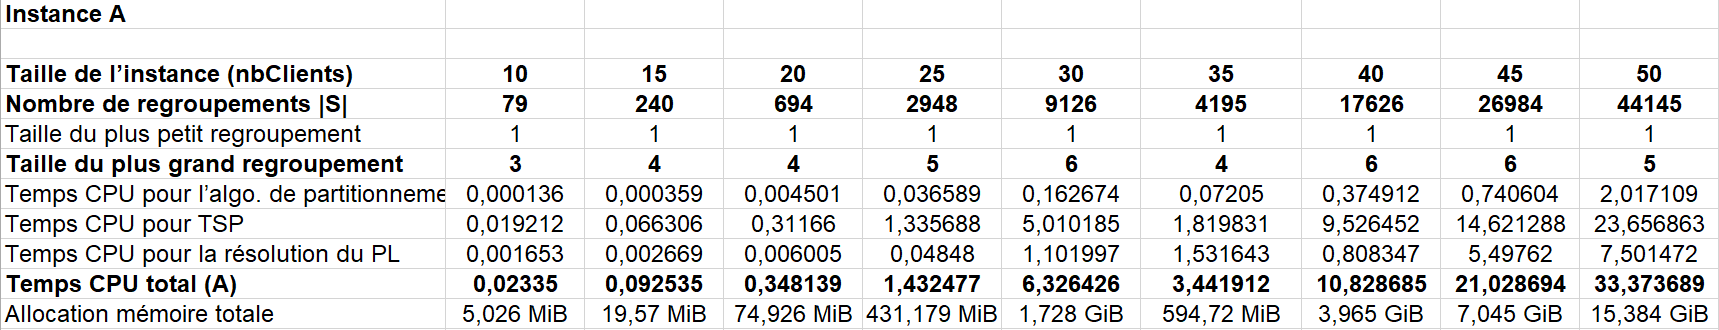
\includegraphics[scale=0.50]{ResExacte_InstA.PNG}
\end{center}

    On note tout d'abord que, pour \verb+nbClients+ $=50$, on a l'ordre de grandeur du temps total CPU attendu : $\approx 30$ secondes.
    \smb Globalement, la fonction de résolution du problème TSP prend le plus de temps à s'exécuter, devant les autres fonctions principales.
    \smb En outre, l'allocation mémoire totale qui est très importante, au détriment du temps d'exécution.
Cette allocation pourrait être moindre, de par un code plus optimisé, une modification du typage (limiter la taille d'encodage d'un entier par exemple),
et une limitation des déclarations de variables. Ceci étant dit, il ne faut pas oublier que le programme linéaire (qu'on écrira "PL" par la suite)
donne lieu à autant de variables $x_j$ qu'il y a de tournées/regroupements. 

\subsection{Instances $B$}

\begin{center}
    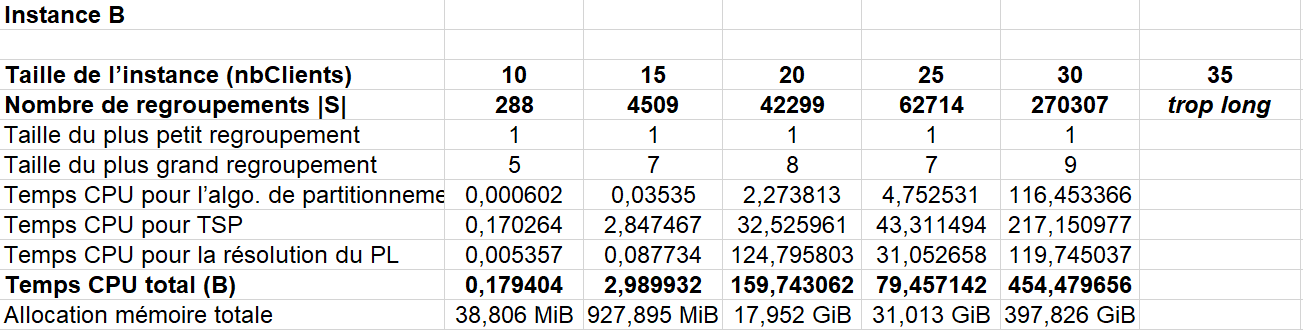
\includegraphics[scale=0.55]{ResExacte_InstB.PNG}
\end{center}

L'exécution sur les instances $B$ prend bien plus de temps. En effet, la capacité y est légèrement supérieure ($capa_A = 30 < capa_B = 33$), et les demandes individuelles ont globalement légèrement diminué.
Par exemple, dans \verb+VRPA15.dat+ (instance $A$ avec \verb+nbClients+ $=15$), on enregistre une demande moyenne de $9,93$,
tandis que dans son homologue $B$, celle-ci atteint $5,4$.
\smb Une telle modification des paramètres implique une accumulation de demandes $\sum_i d_i$ qui s’allonge derrière une capacité plus élevée. D’où davantage de regroupements possibles et de chances d'avoir plus de clients dans un regroupement...
C'est pourquoi, la taille maximale d’un regroupement augmente aussi. Elle croît plus vite pour les instances $B$ que pour les instances $A$.
\smb Enfin, la fonction de partionnement met davantage de temps à s’exécuter : il suffit de regarder la colonne pour \verb+nbClients+ $=30$ pour s’en rendre compte...
Une telle augmentation du nombre de regroupements suggère des traitements plus conséquents dans la fonction \verb+solveTSPExact+ !
Qui dit davantage de tournées, dit davantage de variables $x_j$. Donc la résolution du PL s’effectue également en un temps bien plus conséquent.

\subsection{Analyse graphique et rapports de comparaison}

Puisque la résolution exacte sur les instances de $B$, avec \verb+nbClients+ $>30$, n'aboutit pas en un temps raisonnable,
on se concentre sur les instances $A$ et $B$ dont \verb+nbClients+ $\leq 30$.
Comparons face-à-face les graphiques des temps totaux CPU pour les deux types d'instances :
\begin{center}
    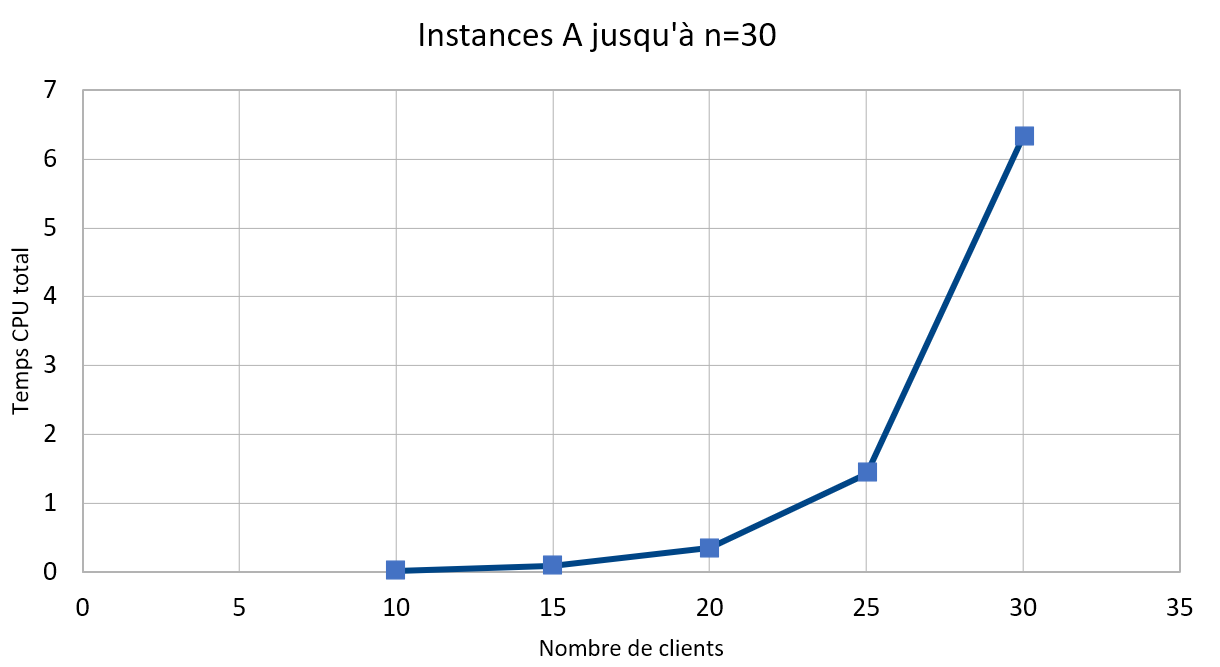
\includegraphics[scale=0.34]{GraphInstA30.PNG}
    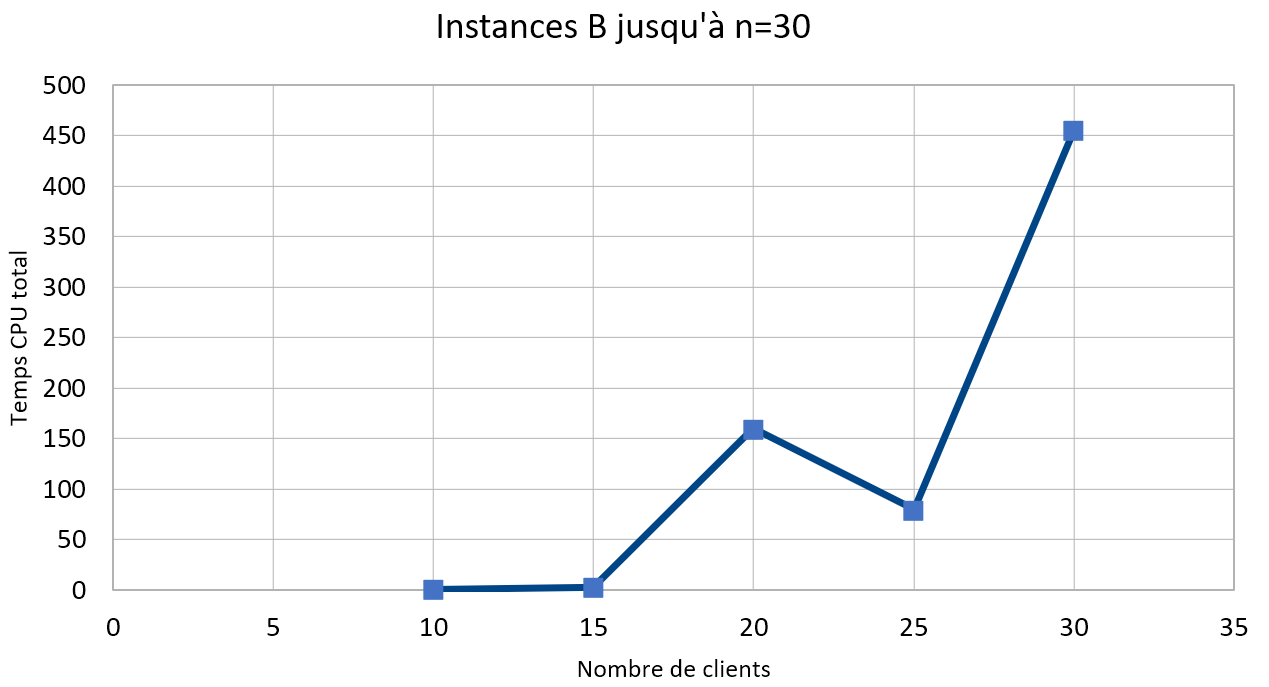
\includegraphics[scale=0.34]{GraphInstB30.PNG}
\end{center}

Le point le plus flagrant à souligner est la différence d'échelle de temps entre les deux graphiques. Celle-ci 
atteste des temps totaux CPU bien plus importants enregistrés pour les instances $B$.
\smb De plus, le temps total CPU pour les instances $A$ semble croître exponentiellement, ce qui n'est pas forcément
le cas pour les instances $B$. En effet, sur le graphique de droite, on note un pic parasite à \verb+nbClients+ $=20$
ainsi qu'une monotonie et une vitesse de croissance très irrégulières (les pics \verb+nbClients+ $\in \{20,30\}$ sont très soudains et les suivants doivent être pires).
Des arguments précédents sur l'analyse des instances $B$ viennent confirmer une évolution du temps CPU aussi singulière.

\smb Enfin, un tableau des rapports des temps totaux CPU et des tailles $|\Sc|$ des regroupements entre les instances $B$ et $A$
est donné à la page suivante :

\begin{center}
    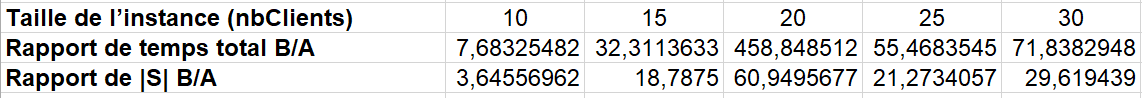
\includegraphics[scale=0.60]{Ratios.PNG}
\end{center}

ainsi que les graphiques témoignant de la croissance de ces rapports (le point parasite \verb+nbClients+ $=20$ est exclu) :
\begin{center}
    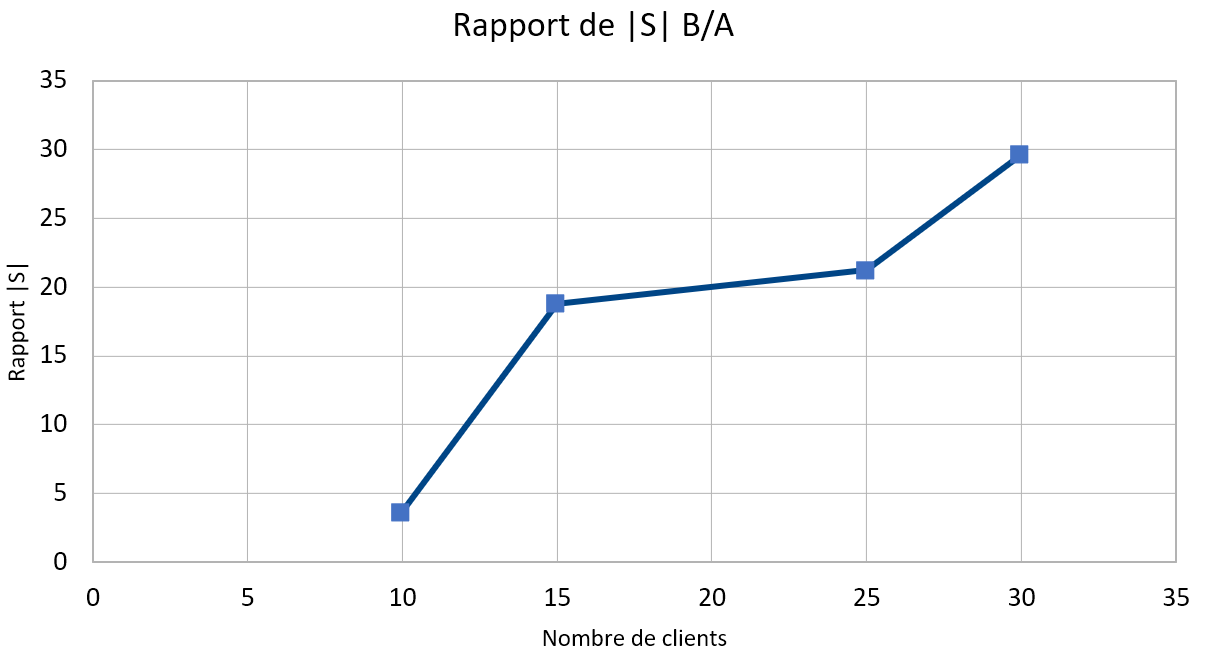
\includegraphics[scale=0.340]{GraphRatioSCallig.PNG}    
    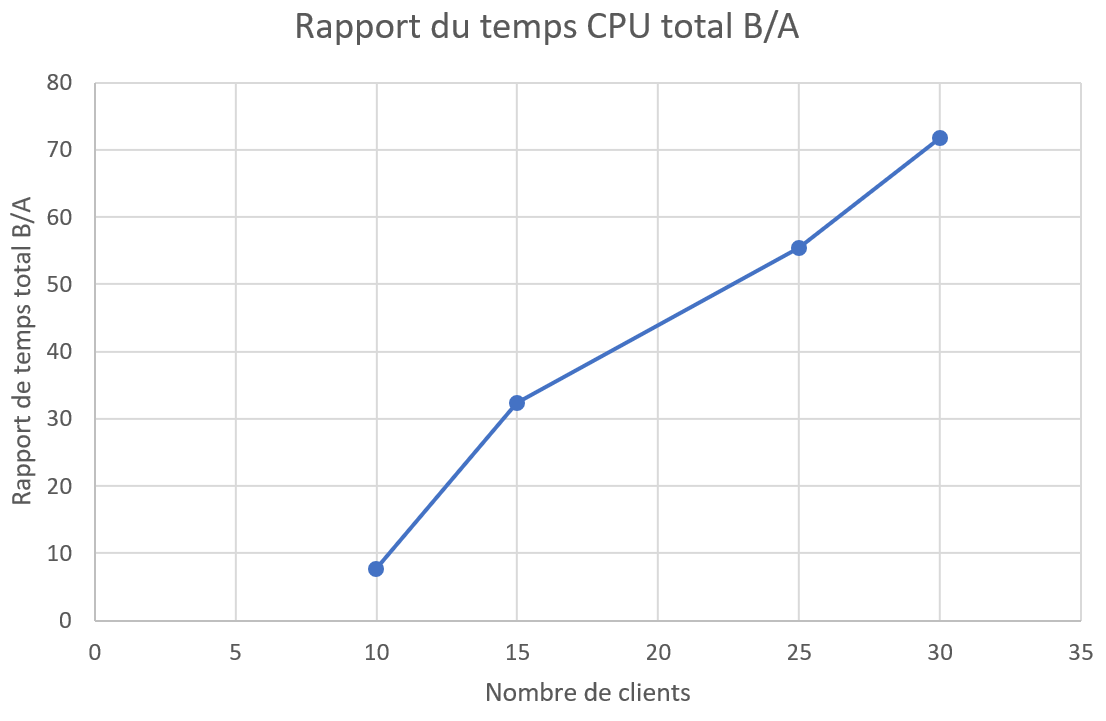
\includegraphics[scale=0.340]{GraphRatioTps.PNG}
\end{center}

Selon les données de l'instance, les regroupements peuvent être complètement différents, ce qui explique
l'allure peu pertinente du graphique de gauche.
\smb Cependant, à droite, le rapport du temps CPU est quasiment proportionnel (si \verb+nbClients+ $=10$ est l'origine)
au nombre de clients. Ainsi, malgré tout, on peut se permettre d'approcher ce constat par : \\ $\exists \alpha \in \R \: : \forall n = \texttt{nbClients} \in \N,$
\[ \dfrac{t_{\text{total},B}(n)}{t_{\text{total},A}(n)} \approx \alpha \cdot n , \]
ce qui témoigne d'une évolution cohérente et raisonnable du temps total CPU en passant d'un type d'instance à un autre.


\subsection{Premières conclusions}
De légères modifications des données (demandes et capacité) entre les instances suffisent à faire gonfler
le nombre de regroupements possibles, à étendre les tournées,
et ainsi à impacter sévèrement les temps CPU, notamment dans la résolution du TSP.
\smb Il est clair que, pour répondre en un temps court aux décideurs, la résolution approchée semble plus
appropriée pour certaines instances telles que celles de type $B$. Voyons dans quelle mesure
cette méthode est qualitative et pertinente.

\section{Qualité de la solution admissible obtenue par la méthode \emph{approchée}}

Il est clair que les fonctions de la méthode approchée donnent des solutions admissibles (par l'heuristique de Clark et Wright)
en un temps très court, voire instantané devant les temps enregistrés pour la méthode exacte.
Pour autant, doit-on être prudent en donnant ces solutions aux décideurs ?
\smb En annexe sont donnés les résultats obtenus pour chaque instance et chaque méthode.
On se focalise sur un comparatif statistique entre le nombre de tournées, la valeur de la fonction objectif
(minimisation de la longueur totale), 
ainsi que l'erreur relative 
(égale à $100 \times \dfrac{z_{\text{exacte}} - z_{\text{approchée}}}{z_{\text{exacte}}}$) :

\begin{center}
    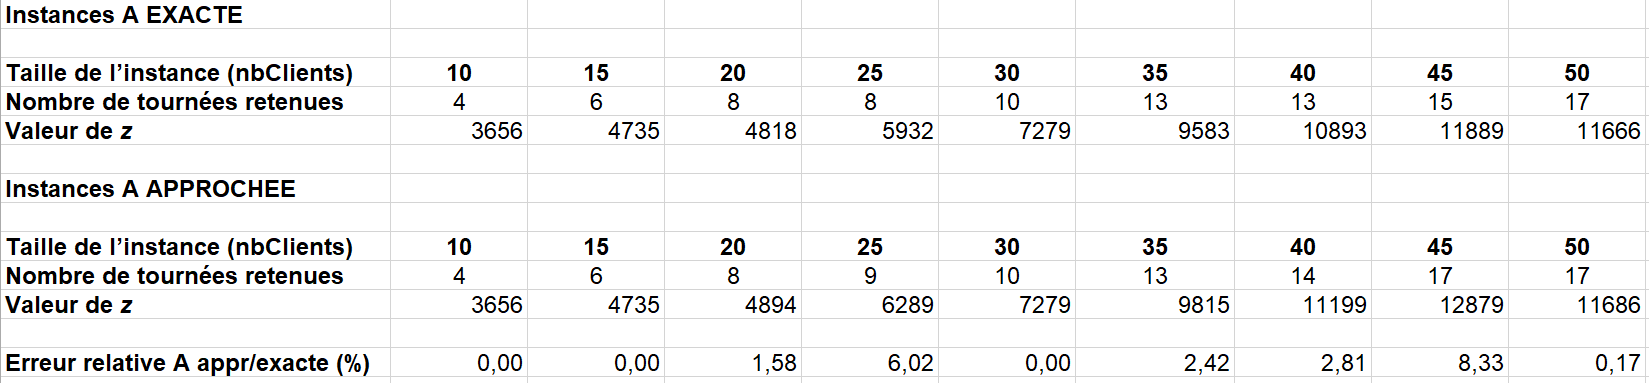
\includegraphics[scale=0.50]{AnalyseInstA.PNG}
    \\
    \vspace{+0.5cm}
    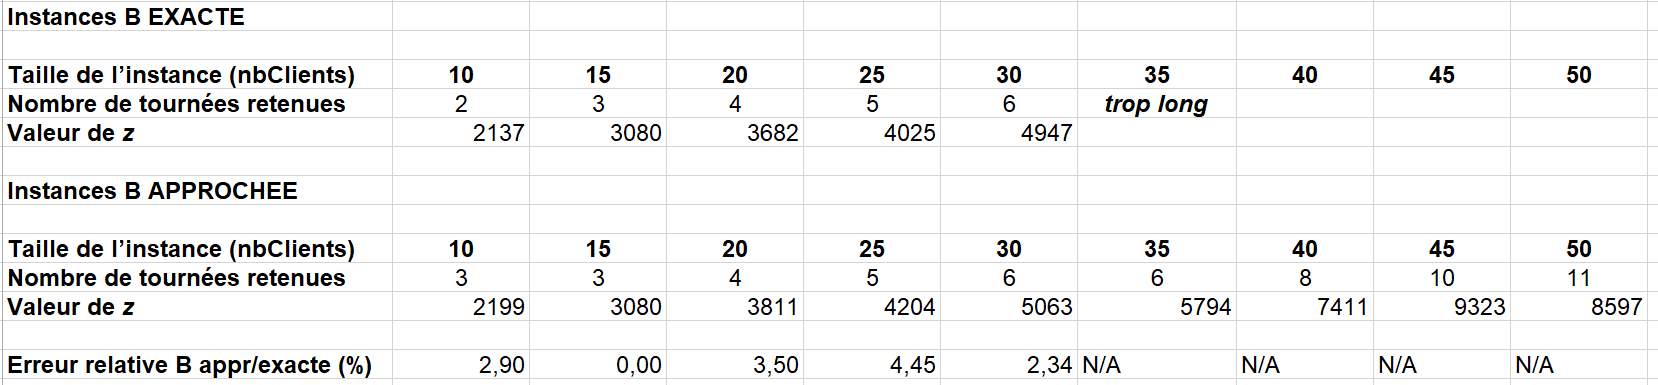
\includegraphics[scale=0.50]{AnalyseInstB.PNG}
\end{center}

On remarque le nombre de tournées retenues par l'heuristique
se rapproche (pour ne pas dire "est égal") de celui par la méthode exacte. Ici, on peut compter au plus
une tournée supplémentaire retenue par la méthode approchée, ce qui est acceptable.

\smb En outre, pour les deux types d'instances, l'erreur relative est très raisonnable : proche de $0$,
du moins inférieure à $10 \%$.

\smb En définitive, pour ces exemples, on peut raisonnablement confier ces solutions admissibles aux décideurs. 
Cependant, est-ce toujours le cas sur d'autres instances, plus grandes, ou plus complexes
(demandes très hétérogènes, ou encore capacité plus ou moins grande) ?

\smb Il faudrait étendre l'analyse à celle de sensibilité. Grâce aux intervalles de sensibilité des coefficients $l_j$
de la fonction objectif, on serait en mesure de préciser si la solution approchée est optimale ou non.

\smb De plus, on peut fournir des solutions approchées aux décideurs, avec prudence, grâce à des intervalles de confiance
(inférence statistique). Soit $p$ la probabilité que la solution approchée soit aussi bonne que la solution exacte.
Pour une même instance, on peut comparer un échantillon de $n$ solutions exactes optimales
et un échantillon de $n$ solutions approchées, puis construire un intervalle de confiance de niveau $1-\alpha$ ($\alpha \in (0,1)$) pour la probabilité $p$.

\section{Conclusion}

La méthode exacte a montré qu'elle présentait ses faiblesses devant certaines instances, telles que celles de type
$B$ de grande taille, qui conféraient des temps d'exécution très conséquents. Ces derniers ne peuvent pas être
tolérés par les décideurs qui veulent une solution admissible en un temps raisonnable, notamment
dans un tel contexte de pandémie. On peut cependant reconnaître que les algorithmes écrits pour la méthode exacte
peuvent être encore optimisés, ce qui aurait pu dégager davantage de solutions optimales (pour \verb+nbClients+$_B > 30$).
\smb Ainsi, comme l'ont montré les instances fournies, 
la méthode approchée fournit aux décideurs des solutions de bonne qualité,
quasiment instantanément. Néanmoins, pour s'en assurer, il faudrait faire une analyse plus poussée,
expérimenter sur d'autres instances, et faire preuve de prudence en donnant des solutions admissibles
approchées.




\newpage

\section*{Annexe : comparaison détaillée des tournées retenues selon la méthode optée}

\end{document}
%% fin
